\chapter{La trave}


\section{Introduzione}
La meccanica delle strutture si propone di modellare corpi che sono in qualche modo sottili, poiché una delle loro dimensioni è marcatamente inferiore alle altre due, come nel caso di piastre e gusci, o perché due dimensioni sono più piccole della terza, come nel caso di cavi e travi. La peculiarità della sottigliezza di una o dell'altra classe di corpi viene sfruttata per assemblare modelli matematici a dimensione ridotta, bidimensionali nel caso di piastre e gusci e monodimensionali per cavi e travi.

Le teorie strutturali  trovano applicazioni estese  nel campo della biomeccanica, dove vengono utilizzate per modellare e analizzare il comportamento meccanico di strutture biologiche complesse.
Ci occuperemo in particolare delle travi che, in questo contesto, rappresentano ossa, legamenti e altre componenti del corpo umano che, sotto l'azione di forze esterne, subiscono deformazioni. L'obiettivo principale è comprendere come queste strutture reagiscano ai carichi, permettendo così di migliorare la diagnosi e il trattamento di patologie muscoloscheletriche, progettare protesi e dispositivi ortopedici più efficienti, e contribuire alla biomeccanica sportiva per prevenire infortuni e ottimizzare le prestazioni.


\section{Geometria}
 Nella configurazione di riferimento, un corpo a forma di trave (a sezione uniforme) è una regione cilindrica con diametro\footnote{Ricordiamo che il \textit{diametro} di un insieme di punti  $\Sc$ è la massima distanza  tra due punti dell'insieme:
 	$$
 	\textrm{diam}\, \Sc\coloneqq\sup_{(\xb, \zb)\in\Sc}|\xb-\zb|.
 	$$
 } molto più piccolo della lunghezza del cilindro. Denotiamo con
 \begin{equation}
 	\Tc=\Sc \times (0,\ell)
 \end{equation}
 questa regione; $\Sc \in \Ec^2$ è la \textit{sezione trasversale} e $\ell$ la \textit{lunghezza} della trave, con
\begin{equation}
	\textrm{diam}\,\Sc\ll \ell
\end{equation}
Scegliamo una volta per tutte nello spazio Euclideo tridimensionale una base cartesiana $\{\eb_i\}$ ($i=1,2,3$) e un'origine.  Fissiamo gli assi in modo che l'origine sia contenuta in $\Sc$ e associamo ai vettori della base un sistema di coordinate $\{x_1, x_2, x_3\}$.
%;  useremo indifferentemente anche il sistema di coordinate $\{x_1, x_2, z\}$, con $x\equiv x_1$, $y\equiv x_2$ e $z\equiv x_3$.  
Vista la geometria di $\Tc$, il suo  generico punto\footnote{Qui e nel seguito pedici indicati con lettera greca sono da intendersi come 1 o 2, a differenza di quelli con lettera latina, che sono da intendersi come 1,2 o 3. }
\begin{equation}
	\xb =x_\alpha \eb_{\alpha}+x_3 \eb_3\equiv x_1\eb_1+x_2\eb_2+x_3\eb_3
\end{equation}
può essere convenientemente decomposto come
\begin{equation}
\xb=\pb+x_3 \eb_3,
\end{equation}
dove $\pb\coloneqq (\xb\cdot\eb_{\alpha})\eb_{\alpha}=x_1 \,\eb_1+x_2\,\eb_2$ è la proiezione di $\xb$ sulla sezione trasversale.

 L'insieme
\begin{equation}
\Lc\coloneqq \{ \xb \in \Tc \,|\, \xb\cdot\eb_{\alpha} =0  \}
\end{equation}
 rappresenta l'\textit{asse} della trave. La frontiera di $\Tc$ è costituita dal \textit{mantello}
 \begin{equation}
 	\Mc\coloneqq\partial \Sc \times (0, \ell)
 \end{equation}
 e dalle \textit{basi}
 \begin{equation}
\Bc_0\coloneqq \Sc\times\{0\}, \qquad \Bc_\ell\coloneqq \Sc\times\{\ell\}.
 \end{equation}
 
 

\section{Il campo di spostamento}
Il modello di trave che intendiamo costruire si caratterizza, oltre che per una speciale geometria, per la selezione di una particolare classe di spostamenti e deformazioni che si considera, meno ricca di quella di un generico corpo tridimensionale, ma sufficientemente ricca da descrivere sommariamente il comportamento di un corpo snello, come è una trave.

In particolare, si assume che in una deformazione ammissibile valgano le seguenti ipotesi:
\begin{enumerate}[label=(H\arabic*)]
	\item  le sezioni $\Sc$ si mantengono piane;
	\item le sezioni $\Sc$  sono rigide e dunque la loro geometria non varia.
\end{enumerate}

Come vedremo, il campo di spostamento tridimensionale $\hat\ub$, definito in $\Tc\ni\xb=\pb+x_3\eb_3 $ che rispetta le ipotesi sopra elencate ha la seguente forma:
\begin{definition}
	\begin{equation}\label{u3d}
\hat\ub(\pb, x_3)=\ub(x_3)+\varthetab(x_3)\times\pb.
\end{equation}
\end{definition}
Una nuova configurazione del cilindro $\Tc$ è così determinata dai campi vettoriali $\ub(x_3)$ e $\varthetab(x_3)$ definiti sull’asse $\Lc$; questi sono i \textit{descrittori cinematici} del modello di trave, anche detti \textit{spostamenti generalizzati}.

\begin{figure}[h!]
	\centering
	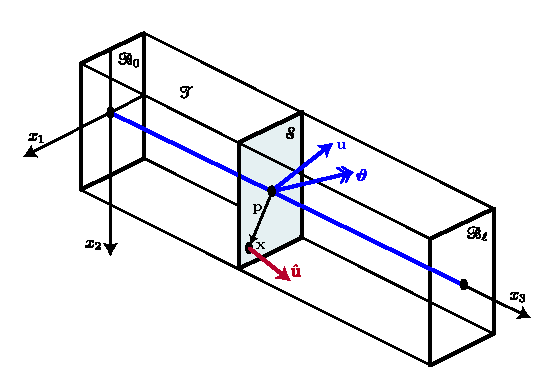
\includegraphics[scale=1.4]{figure/cinematica/trave}
	\caption{Corpo tridimensionale a forma di trave.}
	\label{fig:trave}
\end{figure}



 Il campo $\ub(x_3)$ descrive lo spostamento della linea d'asse e conviene decomporlo come
\begin{definition}
	\begin{equation}
\ub(x_3)=\vb(x_3)+w(x_3)\eb_3, \qquad w(x_3)\coloneqq\ub(x_3)\cdot \eb_3, \;\; \vb(x_3)\coloneqq\ub(x_3)-w(x_3)\eb_3,
\end{equation}
\end{definition}
dove $w(x_3)$ rappresenta il campo di spostamento \textit{longitudinale} della linea d'asse, mentre $\vb(x_3)=v_1 (x_3)\,\eb_{1}+v_2 (x_3)\,\eb_{2}$ lo spostamento \textit{trasversale} della linea d'asse, avente componenti $v_1$ e $v_2$  nelle direzioni $\eb_1$ e $\eb_2$.

La componente $\varthetab(x_3)\times\pb$ di $\hat\ub(\pb, x_3)$ rappresenta una rotazione infinitesima attorno ad un asse parallelo a $\varthetab(x_3)$ e passante per l'asse in $z$.  Anche di $\varthetab(x_3)$ conviene dare la decomposizione:
\begin{definition}
	\begin{equation}
\varthetab(x_3)=\varphib(x_3)+\vartheta(x_3)\eb_{3}, \qquad \vartheta(x_3)\coloneqq\varthetab(x_3)\cdot\eb_3,  \;\; \varphib(x_3)\coloneqq \varthetab(x_3)-\vartheta(x_3)\eb_{3};
\end{equation}
\end{definition}
 vettore $\vartheta(x_3)\eb_3\times \pb$ rappresenta una rotazione infinitesima di $\vartheta(x_3)$ attorno a $\eb_3$, mentre $\varphib(x_3)\times\pb$ rappresenta una rotazione infinitesima attorno ad un vettore diretto come $\varphib(x_3)=\varphi_1 \,\eb_1+\varphi_2\,\eb_2$, perpendicolare alla linea d'asse, e avente componenti $\varphi_1$ e $\varphi_2$ nelle direzioni $\eb_1$ e $\eb_2$.
 
 Possiamo quindi riscrivere   il campo di spostamento tridimensionale come
 \begin{equation}
 	\begin{aligned}
 		\hat{\ub}(x_1,x_2,x_3)
 		%&=\vb(x_3)+w(x_3)\eb_3+\varphib(x_3)\times\pb +\vartheta(x_3)\eb_3 \times \pb \\
 		=\big(v_1(x_3)-x_2 \vartheta(x_3)\big)\eb_1+\big( v_2(x_3)+x_1 \vartheta(x_3) \big)\eb_2+\big( w(x_3)+x_2 \varphi_1(x_3)-x_1\varphi_2 \big)\eb_3.
 	\end{aligned}
 \end{equation}
 
 Il contributo assiale allo spostamento 
\begin{equation}
\hat{u}_3=	w+x_2 \varphi_1-x_1\varphi_2 
\end{equation}
è illustrato in Fig. \ref{fig:travespassiali}.
 
\begin{figure}[h!]
	\centering
	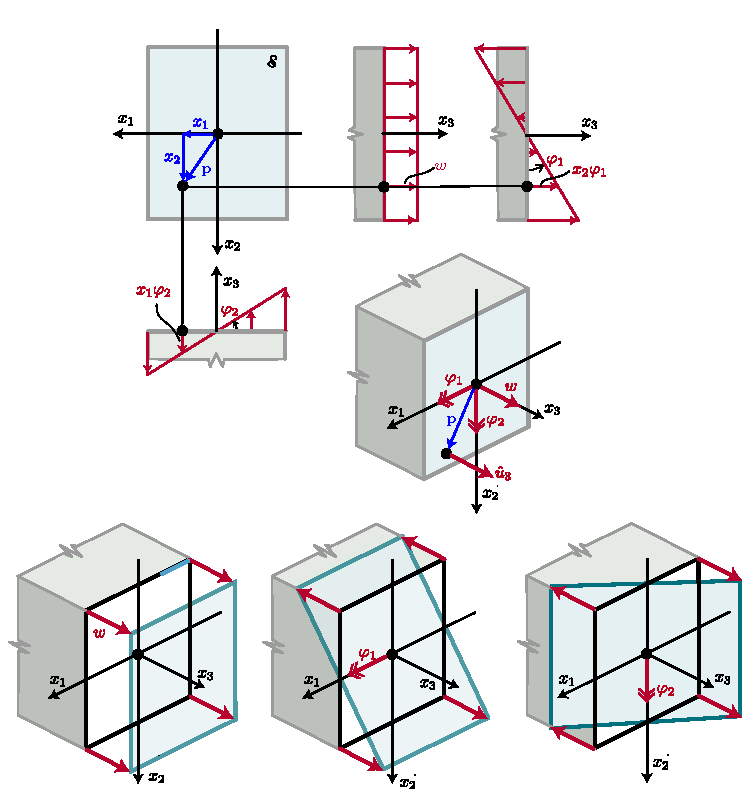
\includegraphics[scale=1.3]{figure/cinematica/trave_sp_assiali}
	\caption{Contributi allo spostamento assiale.}
	\label{fig:travespassiali}
\end{figure}
 
 Il contributo degli spostamento trasversali
 \begin{equation}
 	\hat{u}_1=	v_1-x_2 \vartheta, \qquad  	\hat{u}_2=v_2+x_1 \vartheta
 \end{equation}
 è illustrato in Fig. \ref{fig:travesptrasversali}.
 
 \begin{figure}[h!]
 	\centering
 	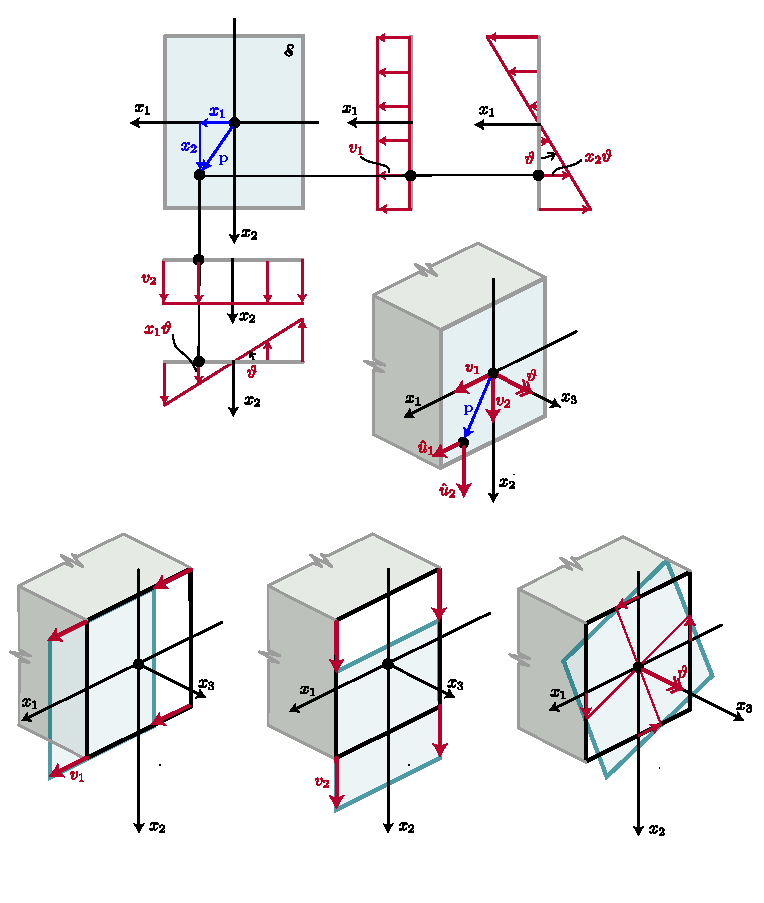
\includegraphics[scale=1.3]{figure/cinematica/trave_sp_trasversali}
 	\caption{Contributi  allo spostamento trasversale.}
 	\label{fig:travesptrasversali}
 \end{figure}

\section{Le misure di deformazione}
Analizziamo adesso quali siano le deformazioni indotte dal campo di spostamento $\hat{\ub}(\pb, x_3)$, verificando che soddisfano le ipotesi (H1) e (H2).
Calcoliamo il gradiente dello spostamento:
\begin{equation}
	\begin{aligned}
\Hb(x_1,x_2,x_3)&=\vartheta(x_3)(-\eb_1\otimes\eb_2+\eb_2\otimes\eb_1)+\big(v_1'(x_3)-x_2\vartheta'(x_3)\big)\eb_1\otimes \eb_3\\
&+\big(v_2'(x_3)+x_1\vartheta'(x_3)\big)\eb_2\otimes \eb_3-\varphi_2\,\eb_3\otimes\eb_1+\varphi_1\,\eb_3\otimes\eb_2\\
&+\big( w'(x_3)+x_2 \varphi_1'(x_3)-x_1\varphi_2'(x_3) \big)\eb_3\otimes\eb_3
\end{aligned}
\end{equation}
e il tensore della deformazione infinitesima:
\begin{equation}
	\begin{aligned}
\Eb(x_1,x_2,x_3)&=\frac12 \big( v'_1(x_3)-\varphi_2(x_3)-x_2\vartheta'(x_3) \big)(\eb_1\otimes\eb_3+\eb_3\otimes\eb_1)\\
&+\frac12 \big( v'_2(x_3)+\varphi_1(x_3)+x_1\vartheta'(x_3) \big)(\eb_2\otimes\eb_3+\eb_3\otimes\eb_2)\\
&+\big( w'(x_3)+x_2 \varphi_1'(x_3)-x_1\varphi_2'(x_3) \big)\eb_3\otimes\eb_3.
\end{aligned}
\end{equation}
Risulta dunque che
\begin{equation}
	E_{11}=E_{22}=E_{12}=0,
\end{equation}
ovvero le sezioni trasversali non si deformano, come richiesto dall'ipotesi (H2). 

Nel seguito, per semplificare la notazione scriveremo $x_3\equiv z$.

Se consideriamo un punto dell'asse  $x_1=x_2=0$, vediamo che la deformazione è descritta da
\begin{equation}
\Eb(0,0,z)=\frac{1}{2}\gamma_1(z)\,(\eb_1\otimes\eb_3+\eb_3\otimes\eb_1)+\frac{1}{2}\gamma_2(z)\,(\eb_2\otimes\eb_3+\eb_3\otimes\eb_2)+\kappa_t(z) \eb_3\otimes\eb_3,
\end{equation}
dove si è posto:
\begin{equation}\label{gamkt}
\gamma_1(z)\coloneqq  v'_1(z)-\varphi_2(z), \quad \gamma_2(z)\coloneqq v'_2(z)+\varphi_1(z), \quad \kappa_t(z)\coloneqq\vartheta'(z).
\end{equation}
Diamone un'interpretazione fisica:
\begin{enumerate}
	\item Il campo vettoriale $\gammab\coloneqq \gamma_1\eb_1+\gamma_2\eb_2$ misura lo \emph{scorrimento angolare}, ossia il \emph{difetto di ortogonalità}, fra l'asse della trave e la fibra del piano della sezione di direzione $\vers{\gammab}$. In particolare, il campo $\gamma_1$ rappresenta l'angolo di scorrimento lungo le direzioni 1 e 3, ovvero tra l'asse della trave e la direzione 1 della sezione; analogamente  $\gamma_2$ per le direzioni 2 e 3.
	\item Il campo scalare $\kappa_t$ misura il tasso di  variazione rispetto all'asse $z$  della componente longitudinale $\vartheta$ della rotazione, ossia la ``rapidità'' con cui la sezione trasversale ruota attorno all'asse della trave.  \`{E} quindi una misura dell'\emph{incurvamento torsionale}, o \emph{torsione} del cilindro, e si dirà \emph{curvatura torsionale}. La componente longitudinale $\vartheta$ della rotazione si dirà \emph{torsionale}.
\end{enumerate}

In generale, l'intero campo di deformazione può essere scritto come
\begin{definition}
	\begin{equation}\label{E3D}
	\begin{aligned}
\Eb(x_1,x_2,z)&=\frac{1}{2}\big(\gamma_1(z)-x_2\kappa_t(z) \big)(\eb_1\otimes\eb_3+\eb_3\otimes\eb_1)\\
&+\frac{1}{2}\big(\gamma_2(z)+x_1\kappa_t(z) \big)(\eb_2\otimes\eb_3+\eb_3\otimes\eb_2)\\
&+\big(\varepsilon(z)+x_2\kappa_1(z)-x_1\kappa_2(z)\big)\eb_3\otimes\eb_3,
\end{aligned}
\end{equation}
\end{definition}
dove si è posto
\begin{equation}\label{epsk}
	\varepsilon(z)\coloneqq w'(z), \quad \kappa_1(z)\coloneqq \varphi_1'(z), \quad  \kappa_2(z)\coloneqq \varphi_2'(z).
\end{equation}
Diamo anche di questi campi un'interpretazione fisica:
\begin{enumerate}
\item $\varepsilon$ misura l'\emph{elongazione specifica} dell'asse (per $\mathbf{r}=\mathbf{0}$ è infatti $E_{11} \equiv \varepsilon$);
\item $\kappab\coloneqq \kappa_1\eb_1+\kappa_2\eb_2$ misura il tasso di variazione rispetto all'asse $z$ della componente trasversale $\varphib$ della rotazione, ossia la ``rapidità'' con cui la sezione trasversale ruota attorno ad un asse contenuto nel suo piano. \`{E} quindi una misura dell'\emph{incurvamento flessionale}, o \emph{inflessione}, del cilindro e si dirà \emph{curvatura flessionale}. 
La componente trasversale $\varphib$ della rotazione si dirà \emph{flessionale}.
\end{enumerate}

La deformazione della trave è dunque completamente descritta dai campi
\begin{equation}\label{cdd}
	\{ \varepsilon, \quad \gamma_1,  \quad\gamma_2, \quad\kappa_1, \quad\kappa_2, \quad\kappa_t \},
\end{equation}
che rappresentano le \textit{misure di deformazione} di una trave. 

Introducendo i vettori della deformazione
\begin{equation}
\eb\coloneqq \gammab +\varepsilon\,\eb_3,  \qquad \kb\coloneqq \kappab+\kappa_t \eb_3
\end{equation}
possiamo scrivere le \eqref{gamkt} e \eqref{epsk} in maniera compatta:
\begin{definition}
	\begin{equation}\label{congrtr}
\eb=\ub'-\varthetab\times \eb_3,  \qquad \kb=\varthetab'.
\end{equation}
\end{definition}
Il campo di deformazione tridimensionale può essere espresso in termini delle misure di deformazione della trave:
\begin{equation}\label{Etr}
	\Eb=\sym{[(\mathbf{e} + \mathbf{k} \times \mathbf{p}) \otimes \mathbf{e}_3]}.
\end{equation}

Le relazioni  \eqref{congrtr} che  connettono le misure di deformazione agli spostamenti,  hanno lo stesso ruolo della relazione
\begin{equation}
	\Eb = \sym \Hb
\end{equation}
nei corpi tridimensionali di forma qualsiasi. Se pensiamo  che le deformazioni siano \textit{assegnate}, le \eqref{gamkt}  e \eqref{epsk}, che riscriviamo come 
\begin{definition}
	\begin{equation}\label{congr}
	\begin{aligned}
&w'(z)=\varepsilon(z), \quad &&\varphi_1'(z)=\kappa_1(z), \quad  && \varphi_2'(z)=\kappa_2(z) \\
&  v'_1(z)-\varphi_2(z)=\gamma_1(z), \quad && v'_2(z)+\varphi_1(z)=\gamma_2(z), \quad&& \vartheta'(z)=\kappa_t(z),
\end{aligned}
\end{equation}
\end{definition}
sono note come \textit{equazioni di congruenza} per la trave; corredate delle opportune condizioni al contorno, costituiscono il \textit{problema cinematico}, la cui soluzione consente di determinare il campo di spostamento, e dunque la forma della trave, note le caratteristiche della deformazione.

Osserviamo che le caratteristiche della deformazione \eqref{cdd} sono campi definiti sulla linea d'asse, il che rende il modello della trave che stiamo costruendo una teoria di campo monodimensionale e dunque notevolmente più semplice di quella tridimensionale che abbiamo trattato nella sezione precedente; la ricostruzione del campo di deformazione tridimensionale è eventualmente possibile utilizzando la \eqref{E3D}.  Per questa ragione, da un punto di vista grafico, rappresenteremo la trave indicando esclusivamente la sua linea d'asse.



\section{La trave piana}
\lipsum[1]
\begin{definition}
	\begin{equation}\label{congrpiana}
		\begin{aligned}
			&w'(z)=\varepsilon(z), \qquad \varphi'(z)=\kappa(z), \qquad  v'(z)+\varphi(z)=\gamma(z).
		\end{aligned}
	\end{equation}
\end{definition}



\begin{exercise}
	Si consideri una trave piana in figura, su cui siano assegnate le deformazioni $\gamma = \bar{\gamma}>0$, $\varepsilon = 0$ e $\kappa = 0$, si determinino i campi di spostamento $v(z)$, $w(z)$ e $\varphi (z)$.
\begin{center}
	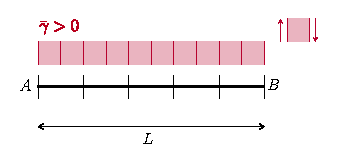
\includegraphics[scale=1.2]{figure/cinematica/esempio1}
\end{center}

\begin{svolgimento}
Integrando le \eqref{congrpiana} si ottiene immediatamente
\begin{equation}
w(z)=w_0, \qquad \varphi(z)=\varphi_0, \qquad v(z)=\bar{\gamma}z-\varphi_0 z+v_0.
\end{equation}
Le costanti indeterminate $w_0$, $v_0$, $\varphi_0$ rappresentano un moto rigido d'assieme. Nella figura sotto, scegliendo $w_0=v_0=\varphi_0=0$ si può visualizzare l'effetto della deformazione pura.
\begin{center}
	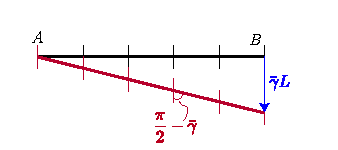
\includegraphics[scale=1.2]{figure/cinematica/esempio1_1}
\end{center}
\end{svolgimento}
\end{exercise}

\begin{exercise}
	Si consideri una trave piana in figura, su cui siano assegnate le deformazioni $\gamma =0$, $\varepsilon = \bar{\varepsilon}>0$ e $\kappa = 0$, si determinino i campi di spostamento $v(z)$, $w(z)$ e $\varphi (z)$.
\begin{center}
	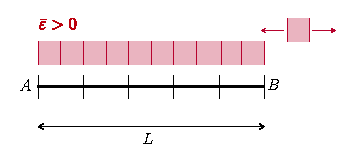
\includegraphics[scale=1.2]{figure/cinematica/esempio2}
\end{center}
\begin{svolgimento}
Integrando le \eqref{congrpiana} si ottiene immediatamente
\begin{equation}
w(z)=\bar{\varepsilon}z+w_0, \qquad \varphi(z)=\varphi_0, \qquad v(z)=v_0-\varphi_0z.
\end{equation}
A meno del solito spostamento rigido d'assieme, la situazione è schematizzata nel disegno sotto.
\begin{center}
	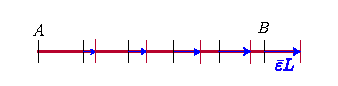
\includegraphics[scale=1.2]{figure/cinematica/esempio2_1}
\end{center}
\end{svolgimento}
\end{exercise}

\begin{exercise}
	Si consideri una trave piana in figura, su cui siano assegnate le deformazioni $\gamma =0$, $\varepsilon = 0$ e $\kappa = \bar{\kappa}>0$, si determinino i campi di spostamento $v(z)$, $w(z)$ e $\varphi (z)$.
	\begin{center}
		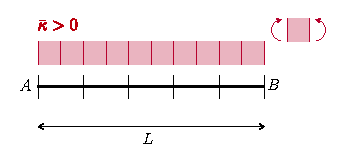
\includegraphics[scale=1.2]{figure/cinematica/esempio3}
	\end{center}
Integrando le \eqref{congrpiana} si ottiene immediatamente
\begin{equation}
w(z)=w_0, \qquad \varphi(z)=\bar{\kappa}z+\varphi_0, \qquad v(z)=-\frac12 \bar{\kappa}z^2-\varphi_0 z+v_0.
\end{equation}
A meno del solito spostamento rigido d'assieme, la situazione è schematizzata nel disegno sotto.
\begin{center}
	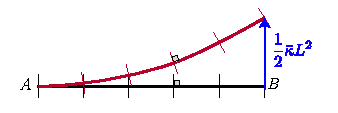
\includegraphics[scale=1.25]{figure/cinematica/esempio3_1}
\end{center}
\end{exercise}

\section{La trave di Eulero-Bernoulli}
In molte circostanze ci si può accontentare di una descrizione della cinematica tridimensionale ancora più semplice di quella proposta dal campo di spostamento \eqref{u3d},  attribuito storicamente a \textsc{S. P. Timoshenko}.
Un modello sovente impiegato in travi molto snelle è  quello che prescrive che le sezioni trasversali si mantengano sempre normali alla linea d'asse. L'ipotesi è detta di \emph{conservazione delle sezioni normali piane} e 
il modello di trave che ne deriva, storicamente attribuito a \textsc{L. Euler} e \textsc{D. Bernoulli}, \`e detto \emph{indeformabile a scorrimento angolare}.
L'indeformabilit\`a a scorrimento angolare equivale dunque a richiedere che 
\begin{definition}
	\begin{equation}
	\gammab=\mathbf{0}.
\end{equation}
\end{definition}
Segue dunque dalle \eqref{congrtr} che 
\begin{equation}\label{Euler}
	\mathbf{v}^{\prime}-\varphib\times\mathbf{e}_3=\mathbf{0}, 
	\quad
	\Rightarrow
	\quad
	\mathbf{v}^{\prime}=\varphib
	\times\mathbf{a},
\end{equation}
da cui, post-moltiplicando vettorialmente per $\eb_3$
\begin{equation}\label{Euler_Cin_30}
	\mathbf{v}^{\prime}\times\mathbf{e}_3=(\varphib\times\mathbf{e}_3)\times\mathbf{e}_3=-\varphib
	\quad
	\Rightarrow
	\quad
	\varphi_1=-v_2^{\prime},
	\quad 
	\varphi_2=v_1^{\prime}.
\end{equation}
Le derivate prime degli spostamenti trasversali all'asse misurano le rotazioni in flessione delle sezioni trasversali: queste non sono pi\`{u} variabili cinematiche 
indipendenti a causa del vincolo  imposto sull'annullarsi dello scorrimento. Le sezioni trasversali ruotano come la tangente all'asse e rimangono ortogonali a essa, e $v_1(z),v_2(z)$ restano quindi i 
soli due descrittori del comportamento trasversale della trave. 
%\begin{figure}[h]
%	\centering
%	\includegraphics[height=2.5cm]{figure/03_cinematica/eulero_bernoulli_c1.pdf}
%	\caption{Cinematica trasversale di travi indeformabili a scorrimento angolare.}
%	\label{fig:EB_10}
%\end{figure}
Per la \eqref{Euler_Cin_30} l'incurvamento in flessione vale
\begin{equation}\label{Euler_Cin_40}
	\kappab=\varphib'=\mathbf{a}\times\mathbf{v}^{\prime\prime}
	\quad
	\Rightarrow
	\quad
	\kappa_1 =-v_2'',
	\, 
	\kappa_2 =v_1''.
\end{equation}
In definitiva, nel modello di trave di Eulero-Bernoulli, gli spostamenti generalizzati indipendenti si riducono a $w, \vb, \vartheta$, le deformazioni generalizzate a $\varepsilon, \kappab, \kappa_t$, le equazioni di congruenza locale si scrivono
\begin{definition}
	\begin{equation}
	\ab \times \vb^{\prime\prime} = \kappab,
	\qquad
	w^\prime = \varepsilon,
	\qquad
	\vartheta^\prime = \kappa_t.
\end{equation}
\end{definition}



%La Fig.~\ref{fig:EB_10} mostra i descrittori cinematici trasversali nei piani $(z, x)$, $(y, z)$ e le sole deformazioni flessionali, in generale diverse da zero. 


Per la trave piana, introdotto il vincolo interno di scorrimento angolare nullo $\gamma = 0$, si ha $\varphi = - v^\prime$ e $\kappa = - v^{\prime\prime}$. 
In questo caso gli spostamenti  indipendenti si riducono a $w, v$, le deformazioni generalizzate a $\varepsilon, \kappa$, le equazioni di congruenza locale si scrivono
\begin{definition}
	\begin{equation}
	- v^{\prime\prime} = \kappa,
	\qquad
	w^\prime = \varepsilon.
\end{equation}
\end{definition}


%\begin{remark}
%	Diversamente dalla deformata della linea d'asse della  trave di Timoshenko, quella di Eulero-Bernoulli non può presentare punti angolosi: eventuali discontinuità degli incurvamenti flessionali ($\kappa_1, \,\kappa_2$)  riguardano infatti le derivate seconde dei campi ($v_1,\, v_2$), e non già le derivate prime,  che invece  risultano continue. 
%\end{remark}

\section{La trave puramente flessibile}

Ci si riduce a questo modello nel caso in cui si assuma che
\begin{equation}
	\eb=\mathbf{0}, \qquad \kappa_t=0.
\end{equation}
In questo caso, oltre alla condizione $\vb^\prime = \varphib \times \ab$ dovuta a $\gammab = \mathbf{0}$, si hanno le condizioni $w^\prime = 0$ e $\vartheta^\prime = 0$ dovute alle richieste che $\varepsilon = 0$ e $\kappa_t = 0$, rispettivamente.
Ne segue che l'unico spostamento generalizzato indipendente è lo spostamento trasversale $\vb$, l'unica deformazione generalizzata ammessa è l'incurvamento flessionale $\kappab$, le equazioni di congruenza si riducono a
\begin{equation}
	\ab \times \vb^{\prime\prime} = \kappab.
\end{equation}



Per la trave piana, introdotte le prescrizioni  di scorrimento angolare nullo $\gamma = 0$ e inestensibilità $\varepsilon = 0$, gli spostamenti generalizzati indipendenti si riducono al solo spostamento trasversale $v$, le deformazioni generalizzate all'incurvamento flessionale $\kappa$, le equazioni di congruenza locale a
\begin{equation}
	-v^{\prime\prime} = \kappa.
\end{equation}


\section{I vincoli}\label{vincolicin}
Per vincoli intendiamo prescrizioni cinematiche  che possono essere assegnate  sugli spostamenti.
Ammettiamo che in un numero finito di punti  $P_j \in \mathcal{C}$ ($j = 1, 2, \ldots$)   della trave è  possibile assegnare delle prescrizioni di natura cinematica, intese come restrizioni indotte da dispositivi comunemente detti \textit{vincoli} costituenti una \emph{giunzione}, da intendersi puntuale, tra la trave e il \textit{suolo}. Per questo parleremo di vincoli posizionali esterni. Considereremo soltanto vincoli \textit{bilateriali} (cioè in grado di assegnare spostamenti in qualunque verso), \textit{scleronomi} (indipendenti dal tempo) e privi di attrito. Il  numero di condizioni scalari che ciascun vincolo impone si chiama \textit{molteciplicità} del vincolo $m$; se $m=1$ il vincolo si dice \textit{semplice}, se $m>1$ \textit{molteplice}.

\subsection{I vincoli spaziali}
Passiamo adesso in rassegna i vincoli spaziali più comuni, assegnando per ciascuno di essi la prescrizione cinematica che impone.
\begin{itemize}
	\item \textit{Appoggio scorrevole su piano di normale $\nb$.} impedisce lo spostamento $\ub$ nella direzione di $\nb$:
	\begin{equation}
		\ub\cdot\nb=0 .
	\end{equation}
	È dunque consentita una traslazione nel piano ortogonale a $\nb$ e la rotazione della sezione trasversale.  Corrispondendo  il vincolo ad una sola condizione scalare, $m=1$; siamo  dunque in presenza di un vincolo semplice.
\item \emph{Appoggio scorrevole su una retta di direzione $\nb$}: impedisce lo spostamento nel piano perpendicolare alla retta:
\begin{equation}
	\ub-(\ub\cdot\nb)\nb=\mathbf{0}.
\end{equation}
È dunque consentita la traslazione nella direzione $\nb$ e la rotazione della sezione trasversale. Corrispondendo il vincolo a due  condizioni scalari, $m=2$.
\item \emph{Cerniera sferica}: impedisce lo spostamento del punto in cui è applicata:
\begin{equation}
	\ub=\mathbf{0}.
\end{equation}
È dunque consentita la sola rotazione della sezione trasversale. Corrispondendo il vincolo a tre  condizioni scalari, $m=3$.
\item \emph{Perno scorrevole di asse $\nb$}: impedisce lo spostamento nel piano perpendicolare a $\nb$, come l'appoggio scorrevole su retta, ma in più impedisce rotazioni della sezione trasversale attorno ad assi perpendicolari ad $\nb$:
\begin{equation}
	\ub- (\ub\cdot\nb)\nb=\mathbf{0}, \quad \varthetab- (\varthetab\cdot\nb)\nb=\mathbf{0}.
\end{equation}
Sono dunque consentiti gli spostamenti nella direzione $\nb$ e le rotazioni della sezione trasversale di asse $\nb$. 
Corrispondendo il vincolo a quattro  condizioni scalari, $m=4$.
\item \emph{Glifo  di asse $\nb$}: impedisce lo spostamento nel piano perpendicolare a $\nb$ e la rotazione della sezione trasversale:
\begin{equation}
	\ub- (\ub\cdot\nb)\nb=\mathbf{0}, \quad \varthetab=\mathbf{0}.
\end{equation}
È dunque consentito il solo spostamento nella direzione $\nb$. Corrispondendo il vincolo a cinque  condizioni scalari, $m=5$.
\item \emph{Cerniera cilindrica di asse $\nb$}: impedisce lo spostamento del punto in cui è applicata e rotazioni della sezione trasversale attorno ad assi perpendicolari ad $\nb$:
\begin{equation}
	\ub=\mathbf{0}, \quad \varthetab- (\varthetab\cdot\nb)\nb=\mathbf{0}.
\end{equation}
È dunque consentita la sola rotazione della sezione trasversale attorno all'asse $\nb$. Corrispondendo il vincolo a cinque  condizioni scalari, $m=5$.
\item \emph{Incastro}: impedisce ogni spostamento generalizzato:
\begin{equation}
	\ub=\mathbf{0}, \quad \varthetab=\mathbf{0}.
\end{equation}
Corrispondendo il vincolo a sei  condizioni scalari, $m=6$.
\end{itemize}

\subsection{I vincoli piani}
\begin{itemize}
	\item \emph{Pendolo o carrello di asse $\nb$}:  impedisce lo spostamento nella direzione $\nb$:
	\begin{equation}
		\ub \cdot \nb = 0.
	\end{equation}

\begin{center}
	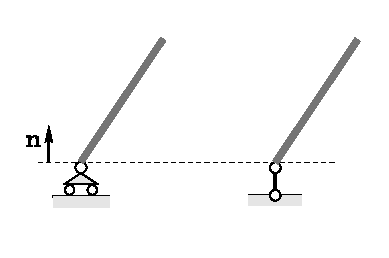
\includegraphics[width=0.4\linewidth]{figure/cinematica/pendolo1}
\end{center}
	È dunque consentito lo spostamento nella direzione perpendicolare a $\nb$ e la rotazione. La molteplicità è $m=1$.
	
	
	\item \emph{Doppio-doppio pendolo} (o \emph{pantografo} o \textit{doppio bipendolo}) : impedisce la rotazione:
	\begin{equation}
		\varphi=0.
	\end{equation}

\begin{center}
	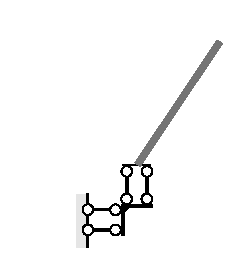
\includegraphics[width=0.25\linewidth]{figure/cinematica/doppiobipendolo1}
\end{center}
	È dunque consentito lo spostamento in ogni direzione. La molteplicità è $m=1$.
	
	
	\item \emph{Glifo (o doppio pendolo o pattino) di asse $\mathbf{n}$}:
	impedisce lo spostamento nella direzione $\nb$ e la rotazione:
	\begin{equation}
		\ub\cdot\nb=0, \quad  \varphi=0.
	\end{equation}
\begin{center}
	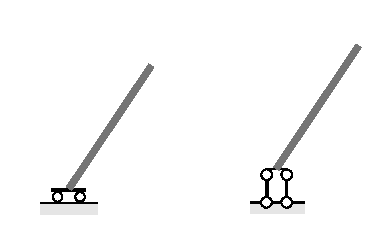
\includegraphics[width=0.4\linewidth]{figure/cinematica/glifo}
\end{center}

	È dunque consentito lo spostamento in direzione perpendicolare a $\nb$. La molteplicità è $m=2$.
	\item \emph{Cerniera}:
	impedisce lo spostamento in ogni direzione:
	\begin{equation}
		\ub = \mathbf{0}.
	\end{equation}
\begin{center}
	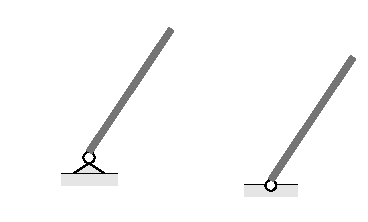
\includegraphics[width=0.4\linewidth]{figure/cinematica/cerniera}
\end{center}
	È dunque consentita la rotazione. La molteplicità è $m=2$.
	
	
	\item \emph{Incastro}: impedisce ogni spostamento generalizzato:
	\begin{equation}
		\ub = \mathbf{0}, \quad \varphi=0.
	\end{equation}
\begin{center}
	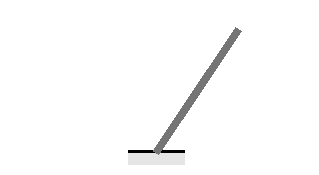
\includegraphics[width=0.35\linewidth]{figure/cinematica/incastro}
\end{center}

	La molteplicità è $m=3$.
\end{itemize}

La presenza di vincoli, alla luce della costruzione di Chasles richiamata nella sezione \ref{spostpiani} basata sulla relazione \eqref{xC}, fornisce delle informazioni su dove si trovino i centri di istantanea rotazione di corpi vincolati.

In particolare, si ha che
\begin{itemize}
	\item Il centro di istantanea rotazione di un corpo vincolato tramite  un carrello di asse $\nb$ si trova su una retta passante per il vincolo e diretta come $\nb$, dato che lo spostamento possibile di quel punto è ortogonale a  $\nb$.
	\item  Il centro di istantanea rotazione di un corpo vincolato tramite un doppio-doppio pendolo di trova in un punto improprio, visto che il corpo non può ruotare.
	\item  Il centro di istantanea rotazione di un corpo vincolato tramite un glifo di asse $\nb$ si trova in nel punto improprio associato alla  direzione $\nb$, avendo quel punto uno spostamento ortogonale a  $\nb$ e non potendo il corpo ruotare. 
	\item  Il centro di istantanea rotazione di un corpo vincolato tramite una cerniera si trova sul vincolo, avendo spostamento nullo.
	\item  Il centro di istantanea rotazione di un corpo vincolato tramite un incastro non esiste.
\end{itemize}


\section{Sistemi di travi}\label{sistr}
I vincoli appena descritti sono da intendersi come dispositivi che collegano un corpo con l'esterno (ad esempio il terreno). Tuttavia è possibile considerare diversi corpi, collegati tra loro da analoghi dispositivi, che denominiamo \textit{vincoli interni}. Le prescrizioni cinematiche rimangono le stesse, ma sono da intendersi come relative tra i corpi, come specificato nella Fig. \eqref{fig:vincoliinterni}.


\begin{figure}[h]
	\centering
	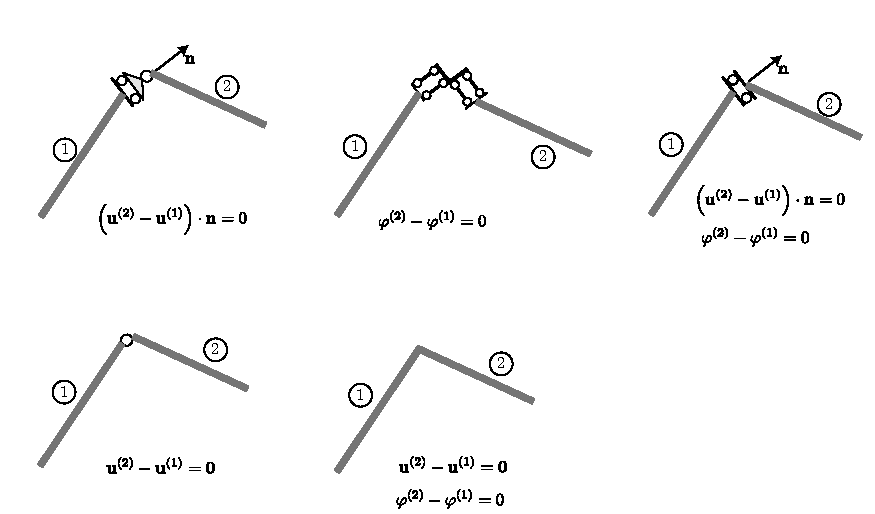
\includegraphics[width=1.1\linewidth]{figure/cinematica/vincoli_interni}
	\caption{Vincoli interni.}
	\label{fig:vincoliinterni}
\end{figure}

Un sistema di travi non è dunque nient'altro che un assemblaggio di travi, collegate tra loro da vincoli interni.

La presenza di più corpi induce all'introduzione della nozione di centro di istantanea rotazione relativa. Dati due corpi $\Omega_1$ e $\Omega_2$, lo spostamento relativo di un punto $\xb$ può essere scritto come
\begin{equation}\label{CR}
\ub^{(12)}=\ub^{(2)}(\xb)-\ub^{(1)}(\xb),
\end{equation}
essendo $\ub^{(1)}$ e $\ub^{(2)}$ i campi di spostamento dei due corpi. Definiamo centro istantaneo di rotazione relativa il punto $\xb_C^{(12)}$ tale che
\begin{equation}
\ub^{(2)}(\xb_C^{(12)})=\ub^{(1)}(\xb_C^{(12)}).
\end{equation}
Valendo la formula di rappresentazione \eqref{urigp}, scegliendo $\xb_0$ coincidente con il centro di rotazione del primo corpo $\xb_C^{(1)}$, possiamo scrivere
\begin{equation}
\ub^{(1)}(\xb_C^{(12)})=\varphi_1 \eb_3 \times (\xb_C^{(12)}-\xb_C^{(1)}),
\end{equation}
essendo $\varphi_1$ la rotazione infinitesima del primo corpo.
Analogamente possiamo procedere per il corpo 2 e stabilire che
\begin{equation}
	\ub^{(2)}(\xb_C^{(12)})=\varphi_2 \eb_3 \times (\xb_C^{(12)}-\xb_C^{(2)}),
\end{equation}
essendo $\varphi_2$ la rotazione infinitesima del secondo corpo.
Vista la definizione di centro relativo \eqref{CR} risulta
\begin{equation}
\varphi_1  (\xb_C^{(12)}-\xb_C^{(1)})=\varphi_2  (\xb_C^{(12)}-\xb_C^{(2)}),
\end{equation}
che, se $\varphi_1\neq \varphi_2$,  può essere riscritta come
%\begin{equation}
%(\varphi_1-\varphi_2 )	\xb_C^{(12)}=\varphi_1\xb_C^{(1)}-\varphi_2\xb_C^{(2)}.
%\end{equation}
%Se $\varphi_1\neq \varphi_2$, otteniamo
%\begin{equation}
%	\xb_C^{(12)}=\frac{\varphi_1\xb_C^{(1)}-\varphi_2\xb_C^{(2)}}{\varphi_1-\varphi_2},
%\end{equation}
%da cui
\begin{equation}
\xb_C^{(12)}-\xb_C^{(1)}=\frac{\varphi_2}{\varphi_1-\varphi_2}\Big(  \xb_C^{(1)} -\xb_C^{(2)}\Big) \qquad \Longrightarrow \qquad \xb_C^{(12)}-\xb_C^{(1)}\parallel \xb_C^{(1)} -\xb_C^{(2)}.
\end{equation}
Vale dunque il 
\begin{definition}
\textit{\textbf{Primo teorema di Aronhold--Kennedy}}. Dati due corpi, il centro di rotazione relativa e i due centri di rotazione assoluta sono allineati.
\end{definition}

Consideriamo adesso tre corpi. Con evidenza dei simboli abbiamo che 
\begin{equation}
		\xb_C^{(12)}=\frac{\varphi_1\xb_C^{(1)}-\varphi_2\xb_C^{(2)}}{\varphi_1-\varphi_2}, \qquad 
			\xb_C^{(13)}=\frac{\varphi_1\xb_C^{(1)}-\varphi_3\xb_C^{(3)}}{\varphi_1-\varphi_3}, \qquad
			\xb_C^{(23)}=\frac{\varphi_2\xb_C^{(2)}-\varphi_3\xb_C^{(3)}}{\varphi_2-\varphi_3}.
\end{equation}
abbiamo allora che 
\begin{equation}
\begin{aligned}
	&\xb_C^{(12)}-\xb_C^{(13)}=\left( \frac{\varphi_1(\varphi_2-\varphi_3)}{(\varphi_1-\varphi_2)(\varphi_1-\varphi_3)} \right)\left(\xb_C^{(1)} -\frac{\varphi_2(\varphi_1-\varphi_3)}{\varphi_1(\varphi_2-\varphi_3)}\xb_C^{(2)}+\frac{\varphi_3(\varphi_1-\varphi_2)}{\varphi_1(\varphi_2-\varphi_3)}\xb_C^{(3)}
\right),\\
&\xb_C^{(13)}-\xb_C^{(23)}=\left( \frac{\varphi_1(\varphi_2-\varphi_3)}{(\varphi_1-\varphi_3)(\varphi_2-\varphi_3)} \right)
\left(\xb_C^{(1)} -\frac{\varphi_2(\varphi_1-\varphi_3)}{\varphi_1(\varphi_2-\varphi_3)}\xb_C^{(2)}+\frac{\varphi_3(\varphi_1-\varphi_2)}{\varphi_1(\varphi_2-\varphi_3)}\xb_C^{(3)},
\right)
\end{aligned}
\end{equation}
e dunque 
\begin{equation}
\xb_C^{(12)}-\xb_C^{(13)}\parallel\xb_C^{(13)}-\xb_C^{(23)}.
\end{equation}

Concludiamo allora che vale  il 
\begin{definition}
	\textit{\textbf{Secondo teorema di Aronhold--Kennedy}}. Dati tre corpi, i centri di rotazione relativi  sono allineati.
\end{definition}

La presenza di vincoli interni tra i corpi fornisce delle indicazioni su dove si trovi il centro relativo, così come accadeva per i vincoli esterni in relazione ai centri assoluti.
In particolare, si ha che
\begin{itemize}
	\item Il centro di istantanea rotazione relativa tra due corpi vincolati tramite  un carrello di asse $\nb$ si trova su una retta passante per il vincolo e diretta come $\nb$, dato che lo spostamento relativo possibile in corrispondenza  di quel punto è ortogonale a  $\nb$.
	\item   Il centro di istantanea rotazione relativa tra due corpi vincolati tramite un doppio-doppio pendolo di trova in un punto improprio, visto che i corpi non possono ruotare uno rispetto all'altro.
	\item   Il centro di istantanea rotazione relativa tra due corpi vincolati  tramite un glifo di asse $\nb$ si trova in nel punto improprio associato alla  direzione $\nb$, subendo quel punto uno spostamento relativo ortogonale a  $\nb$ e non potendo i corpi ruotare uno rispetto all'altro. 
	\item  Il centro di istantanea rotazione relativa tra due corpi vincolati  tramite una cerniera si trova sul vincolo, avendo spostamento relativo nullo.
	\item   Il centro di istantanea rotazione relativa tra due corpi vincolati  tramite un incastro non esiste.
\end{itemize}

L'uso delle considerazione appena esposte, dei due teoremi dei teoremi di  Aronhold--Kennedy e della costruzione di Chasles illustrata nella Sez \ref{spostpiani} consente di determinare agevolmente il campo di spostamento di sistemi di travi (e, in generale, di corpi) caratterizzati dall'avere un grado di libertà complessivo. 

Consideriamo il sistema di due travi sotto rappresentato.


\begin{center}
	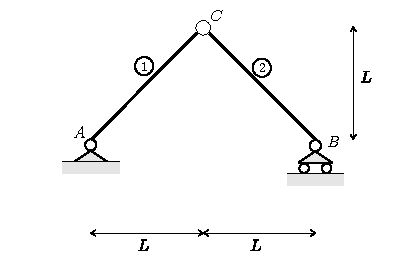
\includegraphics[scale=1.3]{figure/cinematica/biella_manovella}
\end{center}

Essendo vincolato a terra tramite una cerniera in $A$, il corpo 1 ha il centro assoluto $C_1$ in quel punto. La presenza del carrello in $B$ indica che il centro assoluto $C_2$ del secondo corpo si trova su una retta verticale passante per $B$. Infine, la presenza della cerniera in $C$ che collega i due corpi indica che lì si trova il centro relativo $C_{12}$. Dato che i tre centri devono essere allineati, per il primo teorema di Aronhold--Kennedy, il centro di rotazione del secondo è facilmente determinato. A questo punto è immediato rappresentare i diagrammi delle componenti di  spostamento dei due corpi, assumendo ad esempio, che il primo ruoti di un angolo $\varphi$ antiorario, come rappresentato in figura.

\begin{center}
	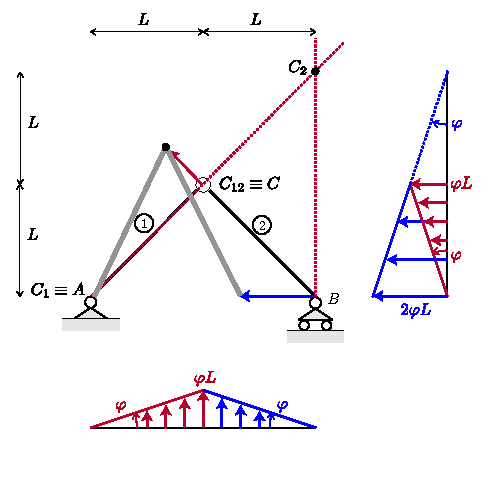
\includegraphics[scale=1.3]{figure/cinematica/biella_manovella1}
\end{center}

I punti $B$ e  $C$ subiscono lo spostamento 
\begin{equation}
\ub(\xb_B)=-2\varphi L \,\eb_1 \qquad  \ub(\xb_C)=\varphi L (-\eb_1+\eb_2)
\end{equation}
I diagrammi delle componenti di spostamento sono rappresentate in rosso per la trave 1 e in blu per la trave 2. In grigio è rappresentata la configurazione deformata a seguito di una rotazione antioraria $\varphi$ della trave 1, che induce ad una rotazione oraria della trave 2 attorno al centro $C_2$, avente della stessa entità $\varphi$.



\textbf{}
